\chapter{Example Printing Workflow}
	
	\label{sec:workflow}
	
	The following appendix contains a walk-through of the complete process of
	designing and printing an object from scratch. The process begins with the
	production of a 3D model of the design. The next step is to convert the model
	into G-code instructions and send them to the printer. A description is then
	given of the key phases of the printing process. Once the print is complete,
	the printed object is ready after a small amount of cleaning if required.
	
	A simple cuboid is used as an example throughout as the process of designing
	complex 3D models is not the focus of this report. The cube will measure
	$20\mm$ wide, $20\mm$ deep and $10\mm$ tall.
	
	\section{3D Modelling (OpenSCAD)}
		
		There are many programs available for 3D modelling but in this example
		OpenSCAD is used. Other tools may be used provided that they can export
		models in the widely used Standard Tessellation Language (STL) file format
		which is accepted by the G-Code generation software shown in this example.
		Alternatively, ready-made models in STL format can be downloaded from
		websites such as Thingiverse \cite{thingiverse}.
		
		OpenSCAD is a constructive-solid-geometry modelling tool that takes
		descriptions of 3D models as text and outputs them as STL files
		\cite{openscad}. In order to define the cube model we specified, the
		following code is used:
		\begin{verbatim}
			cube(size=[20,20,10]);
		\end{verbatim}
		Typing this into the OpenSCAD GUI allows you to see a rendered version of
		the object by choosing `Compile and Render' from the `Design' menu (figure
		\ref{fig:openSCAD}).  The
		object can be exported to an STL file ready for G-code generation by
		choosing `Export as STL' from the same menu.
		
		\begin{figure}
			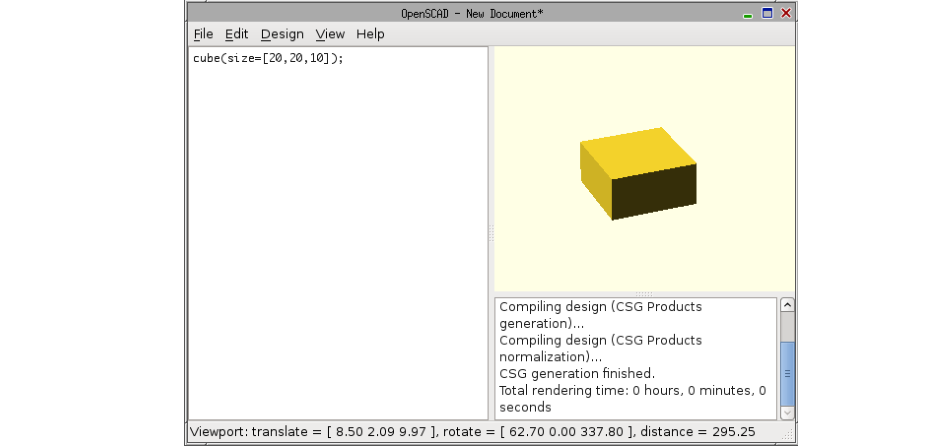
\includegraphics[width=1\textwidth]{diagrams/openSCAD.pdf}
			\caption{OpenSCAD showing a cube model compiled and rendered}
			\label{fig:openSCAD}
		\end{figure}
		
	\section{G-Code Generation (ReplicatorG \& Skeinforge)}
		
		Once an STL file has been produced, G-code for printing the model must be
		generated. ReplicatorG provides a more user-friendly front-end to the
		Skeinforge G-code generator \cite{replicatorg}. Skeinforge relies on a
		calibrated printer profile to guide its decisions. A profile was produced
		compatible with ReplicatorG 27 and Skeinforge 35 as part of the project
		which must be copied into \begin{verbatim}
		replicatorg-0027/skein_engines/skeinforge-35/skeinforge_application/prefs
		\end{verbatim}
		
		Once ReplicatorG has been started, the STL file from the previous step is
		loaded using `Open' from the `File' menu (figure \ref{fig:replicatorG}).
		Once loaded, the model should be positioned centrally on the platform using
		the tools on the right of the preview. Clicking `Move' provides features to
		`Center' the model and `Put on Platform' to ensure the model is not
		printed in mid-air.
		
		\begin{figure}
			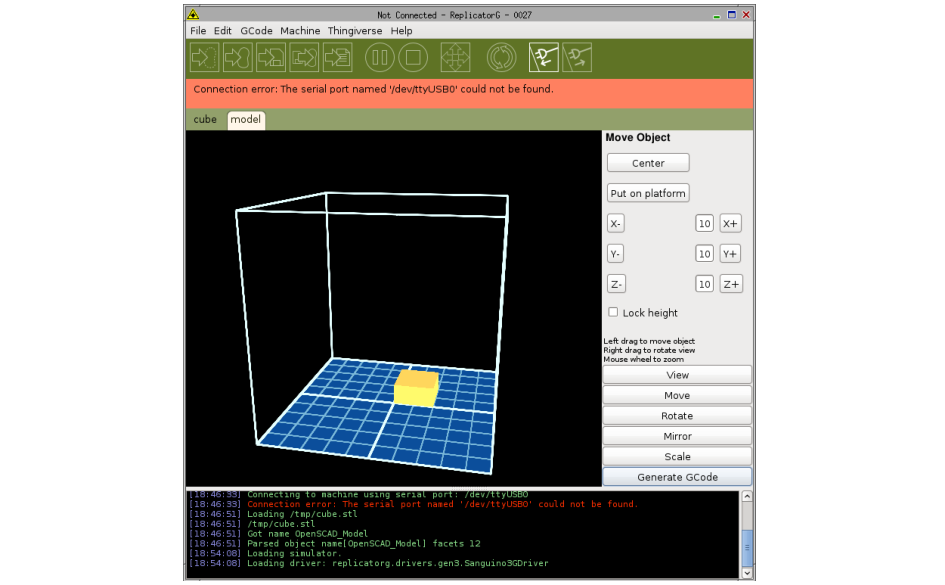
\includegraphics[width=1\textwidth]{diagrams/replicatorG.pdf}
			\caption{ReplicatorG GUI showing a cube model loaded}
			\label{fig:replicatorG}
		\end{figure}
		
		Once the model is correctly positioned, the G-code is generated using the
		`Generate GCode' button. A dialogue will prompt for a profile to be
		selected, `SF35-cupcake-ABP-raftless' should be used (figure
		\ref{fig:skeinforge}). This process can take some time for complex models.
		A \verb|.gcode| file is produced containing the printer data in the same
		directory and with the same name as the STL file.
		
		\begin{figure}
			
\includegraphics[width=1\textwidth]{diagrams/skeinforge.pdf}
			\caption{Skeinforge profile selection dialogue}
			\label{fig:skeinforge}
		\end{figure}
	
	\section{Status Monitoring}
		
		To monitor the printer during a print, a utility called
		\verb|makebed_live.sh| is provided which shows heater temperatures, extruder
		position and buffer usage. It is helpful to have this open during a print to
		monitor the progress of the heating and cooling stages as well as to check
		for buffer underruns.
		
		Figure \ref{fig:makebedlive} (page \pageref{fig:makebedlive}) shows the
		utility in use during a print.
		
	\section{G-Code Streaming}
		
		Before any G-code is sent to the printer, the printer should me moved to its
		`home' position (figure \ref{fig:homing}). This can be done manually by hand
		or automatically by sending a G-code file to the printer containing
		automatic homing instructions\footnote{See appendix \ref{sec:gcode_home_xy}
		for an example of such an automatic homing G-code file.}.
		
		\begin{figure}
			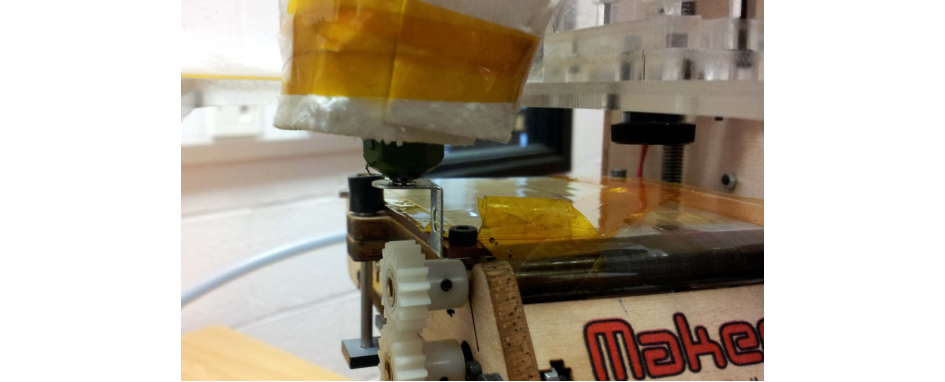
\includegraphics[width=1\textwidth]{diagrams/homing.pdf}
			\caption{Extruder placed in the homing bracket}
			\label{fig:homing}
		\end{figure}
		
		The \verb|makebed.py| utility is used to stream a G-code file to the
		printer:
		\begin{verbatim}
			makebed.py send cube.gcode
		\end{verbatim}
		This command will block until all print data is sent to the printer.
		
		Complete documentation and safety advice for using \verb|makebed.py| to send
		files to the printer is provided in appendix \ref{sec:makebedDoc}.
			
	\section{Printing Process}
		
		The G-code generated by Skeinforge profile created in this project
		goes through several phases during a print. Each of these is described in
		the following subsections.
		
		\subsection{Warm Up \& Self-Clean}
			
			The printer first enables the platform and extruder heaters setting the
			temperatures to $120\dC$ and $225\dC$ respectively. Next, it moves the
			extruder to the heating position, to the left of the platform and in front
			of the rubber cleaning peg. The printer then stays in this position until
			both heaters are up to temperature (taking around 10 minutes).
			
			Some plastic may ooze from the extruder during heating leaving an unknown
			quantity of plastic in the extruder's heating chamber. Before printing,
			the extruder is refilled with plastic and any excess wiped off against the
			cleaning peg (figure \ref{fig:selfClean}).
			
			\begin{figure}
				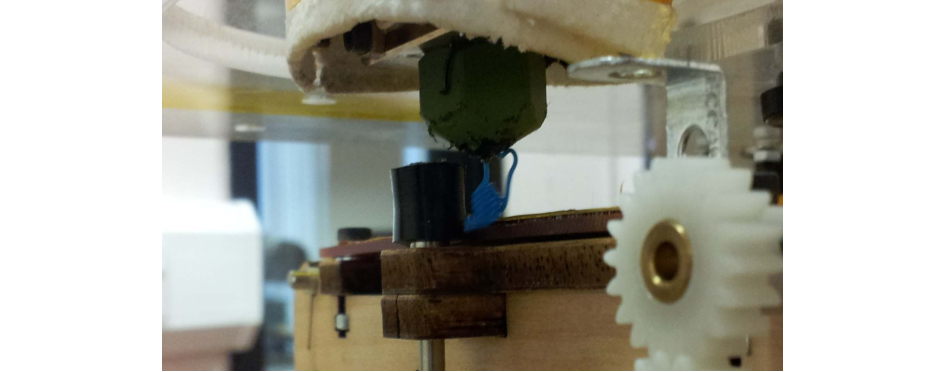
\includegraphics[width=1\textwidth]{diagrams/selfClean.pdf}
				\caption{Extruder extruding plastic during a self-clean}
				\label{fig:selfClean}
			\end{figure}
		
		\subsection{Printing The First Layer}
			
			Once everything has heated up and the extruder is free of excess plastic,
			a rectangle is drawn on the platform which surrounds the area the object
			will be printed in. This allows the operator to check that the print will
			fit on the platform and to allow manual adjustments to the height of the
			extruder to ensure that it is at the correct distance from the bed.
			
			It is critical that the distance between the extruder and platform is
			correct during the printing of the first layer. If it is too far, the
			plastic will not adhere to the platform and will not accurately produce
			the shape required. If it is too close, the plastic printed will not fit
			under the extruder causing the printed object to get caught on the
			extruder as it moves around during the print.
			
			Adjustments should be made by turning the adjustment handle on the Z-axis
			during the printing of the border. The border will be discarded after
			printing and so mistakes can be corrected while it is produced.
			
			Once the border is drawn, the extruder prints out the first layer of the
			object (figure \ref{fig:firstLayer}). This is done at a slower speed than
			other layers allowing more plastic to be deposited producing thicker
			lines helping the print adhere better to the platform.
			
			\begin{figure}
				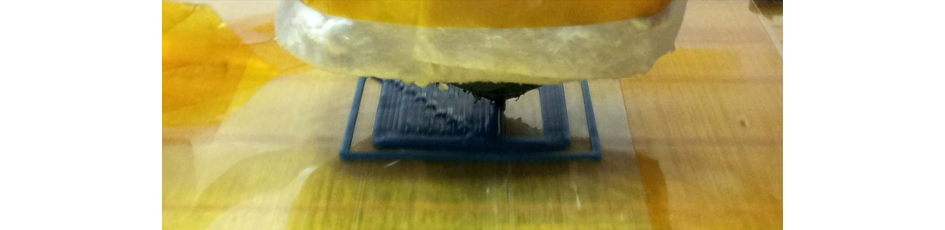
\includegraphics[width=1\textwidth]{diagrams/firstLayer.pdf}
				\caption{First layer being printed}
				\label{fig:firstLayer}
			\end{figure}
			
		\subsection{Main Printing Phase}
			
			During this phase, the model is printed layer by layer. Each layer is
			usually printed first by drawing three solid outer `shells' and then
			filling in the centre. Layers near the top and bottom of the model are
			filled completely to produce a solid finish. Layers inside the model are
			filled with a hexagonal `fill pattern' (figure \ref{fig:fillPattern}). The
			fill pattern is not visible when the object is completed. It is used as it
			significantly reduces the time and plastic required to fill objects while
			still retaining strength.
			
			\begin{figure}
				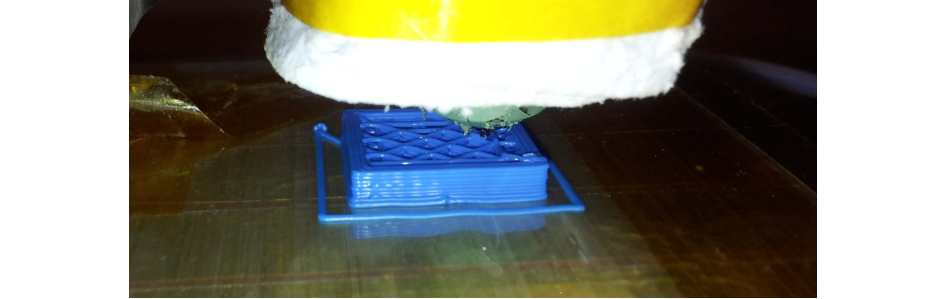
\includegraphics[width=1\textwidth]{diagrams/fillPattern.pdf}
				\caption{Fill pattern being printed}
				\label{fig:fillPattern}
			\end{figure}
			
			The cube takes about 8 minutes to print.
		
		\subsection{Cool-down, Eject and Self-Clean}
			
			Once the print completes, the platform is cooled down to allow
			the object to solidify completely. This takes around 2 minutes.
			
			When the object has cooled, the platform conveyor is activated and the
			object is peeled off the platform and deposited in front of the printer
			(figure \ref{fig:eject}).
			
			\begin{figure}
				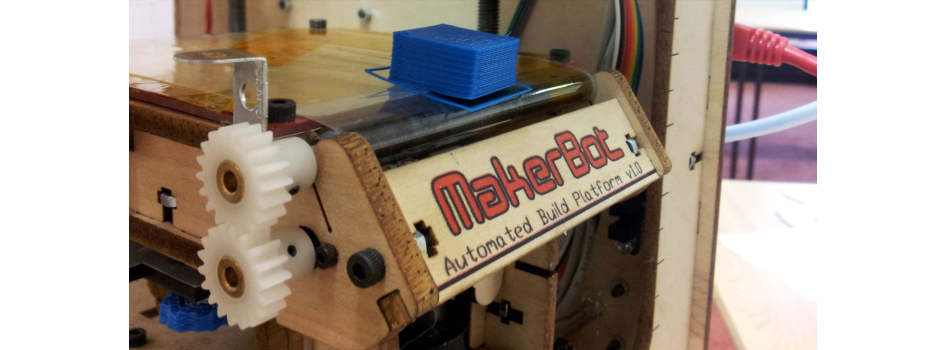
\includegraphics[width=1\textwidth]{diagrams/eject.pdf}
				\caption{Finished cuboid being ejected}
				\label{fig:eject}
			\end{figure}
			
			As plastic oozes out of the extruder after the print completes it must
			once again be cleaned using the same process as the start of the print.
			
			Finally, the printer returns to the home position and the heaters and
			power supply turned off. If another print job is started at this point,
			the extruder will still be hot but the platform, having cooled slightly,
			will need to partly reheated before the print can begin. Many prints can
			be run successively in this way with no human intervention unless a print
			fails.
		
	\section{Final Print}
		
		Once the printer ejects the object it will still be hot and may still be
		slightly soft in some places. Care should be taken when handling the object
		until it has fully cooled.
		
		The border printed at the start can be snapped off and the process is
		complete.  For more complex models, strings of plastic left during printing
		(figure \ref{fig:stringing}) may also need to be removed using a knife.
		
		\begin{figure}
			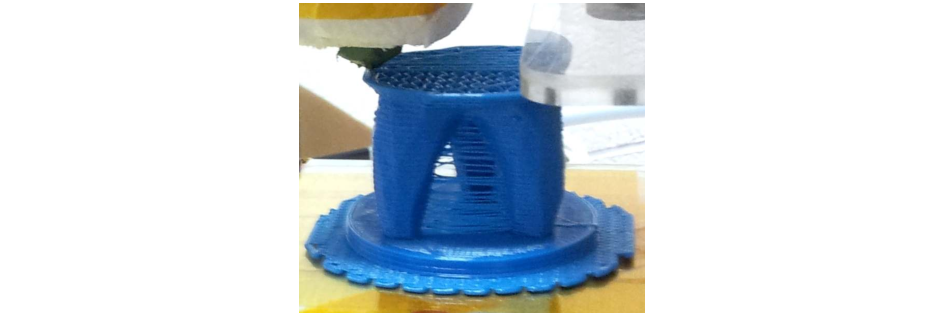
\includegraphics[width=1\textwidth]{diagrams/stringing.pdf}
			\caption{Strings of plastic left during printing requiring manual removal}
			\label{fig:stringing}
		\end{figure}
